\chapter{Implementation Environment}\label{ch:environment}

\section{Hardware and software}

\begin{sidewaysfigure}
  \centering
  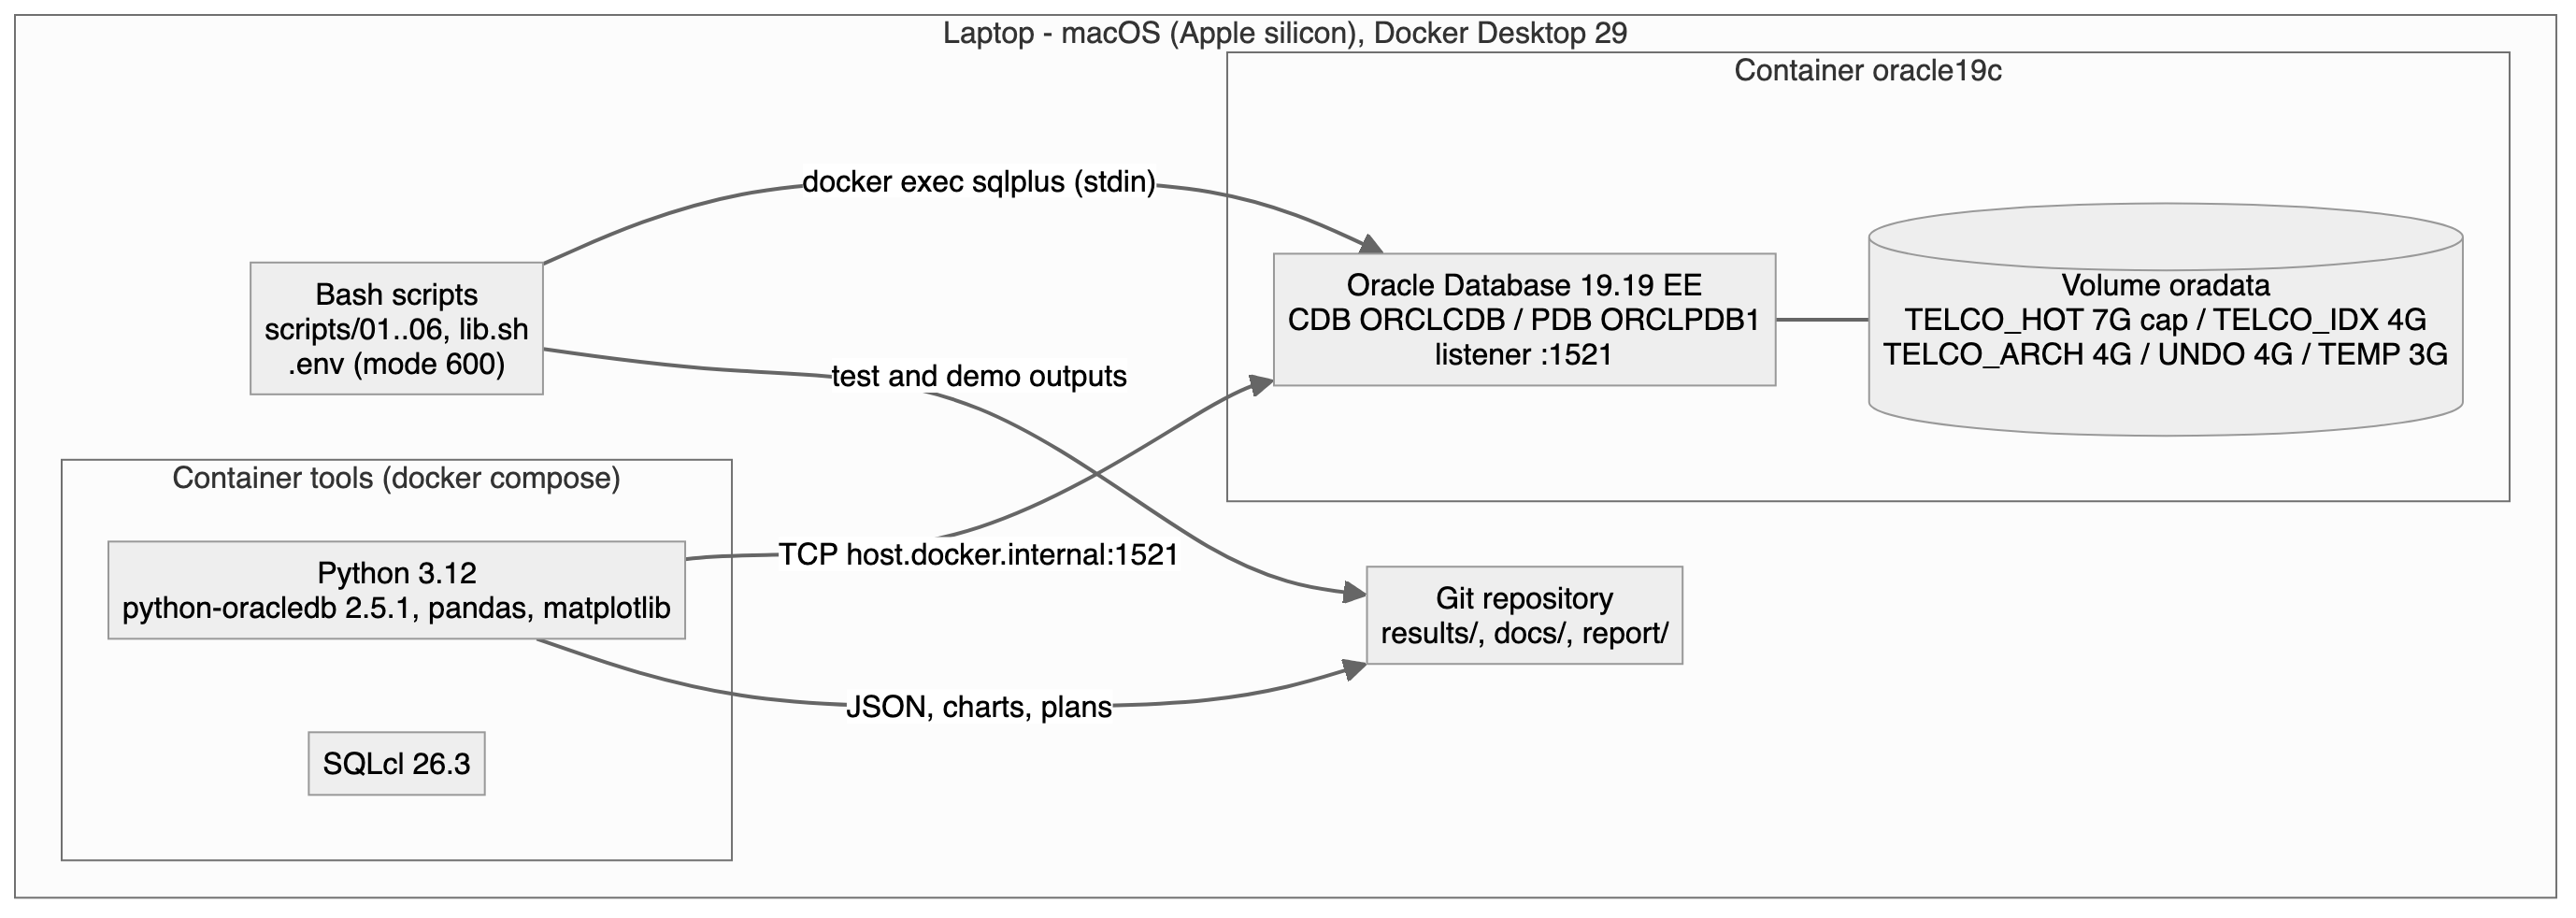
\includegraphics[width=0.9\linewidth]{06_deployment}
  \caption{Deployment diagram}
  \label{fig:deployment}
\end{sidewaysfigure}

Figure~\ref{fig:deployment} shows where each component runs. The database and the tools run in
two containers on the same laptop; the scripts drive SQL*Plus inside the database container
and the benchmark connects over TCP.

\begin{table}[H]
\centering
\caption{Environment and versions}
\begin{tabularx}{\linewidth}{lL}
\toprule
Component & Version / configuration \\
\midrule
Host & Apple silicon laptop, macOS, Docker Desktop 29.0 (8 vCPU, about 8~GB RAM for the Docker VM) \\
Database & Oracle Database 19c Enterprise Edition 19.19 (ARM64), container \code{oracle19c}, CDB \code{ORCLCDB}, PDB \code{ORCLPDB1} \\
Memory & SGA 2.3~GB (buffer cache 1.7~GB), PGA target 784~MB \\
Options & Partitioning (used), Advanced Compression (not used), Diagnostics/Tuning Packs (not used) \\
Tools container & Python 3.12, python-oracledb 2.5.1 (thin), pandas 2.2, matplotlib 3.9, Streamlit 1.40, SQLcl 26.3, OpenJDK 17 \\
Clients & SQL*Plus inside the database container (OS authentication for SYSDBA) \\
Version control & Git, GitHub (\url{\RepoURL}) \\
\bottomrule
\end{tabularx}
\end{table}

\section{Storage configuration}

The laptop disk had only about 20~GB free when the project started, and the defaults of the
course container let UNDO and TEMP grow to 32~GB each. Before generating any data we capped
every file that could grow (Table~\ref{tab:storage}). We also freed about 9~GB by removing
unused Docker images. Every data-loading script checks the free host disk first and stops
below a threshold.

\begin{table}[H]
\centering
\caption{Tablespaces and size caps}
\label{tab:storage}
\begin{tabularx}{\linewidth}{llL}
\toprule
Tablespace & Cap & Content \\
\midrule
\code{TELCO\_HOT} & 7~GB & hot partitions, baseline table, reference data \\
\code{TELCO\_IDX} & 4~GB & indexes of hot data \\
\code{TELCO\_ARCH} & 4~GB & warm and archived partitions (compressed) and their indexes, baseline archive \\
\code{UNDOTBS1} & 4~GB & capped (default 32~GB) \\
\code{TEMP} & 3~GB & capped (default 32~GB) \\
\bottomrule
\end{tabularx}
\end{table}

\section{Prerequisites and installation}

The repository README gives the full procedure, including how to rebuild the Oracle container
from Oracle's official Docker build files. With the container running, the whole solution is
installed by five scripts:

\begin{lstlisting}[style=bash]
scripts/init_env.sh          # .env with random passwords (git-ignored, mode 600)
scripts/01_setup_db.sh       # tablespaces with caps, accounts            [SYSDBA]
scripts/02_create_schema.sh  # tables, views, PL/SQL packages             [TELCO_OWNER]
scripts/03_load_data.sh      # 23.76 M rows over 72 months (about 6 min)
scripts/05_benchmark.sh      # benchmark + report (about 25 min)
\end{lstlisting}

A smoke configuration (3\,000 rows per month) runs the same chain in about one minute and is
used for the destructive functional and security tests (\code{scripts/04\_run\_tests.sh}).

\code{scripts/07\_dashboard.sh} starts the web dashboard (Chapter~\ref{ch:usage}) as a third
Compose service built from the tools image. It listens on \url{http://localhost:8501} only,
and reads the account passwords from \code{.env} without ever displaying them.
